\begin{frame}
    \frametitle{Example events}
    After removing the primary Z boson,
    the \textit{signal} events per channel are interchangeable.
    \centering
    \begin{tabular}{cc}
        \begin{tikzpicture}
          \node (img1) {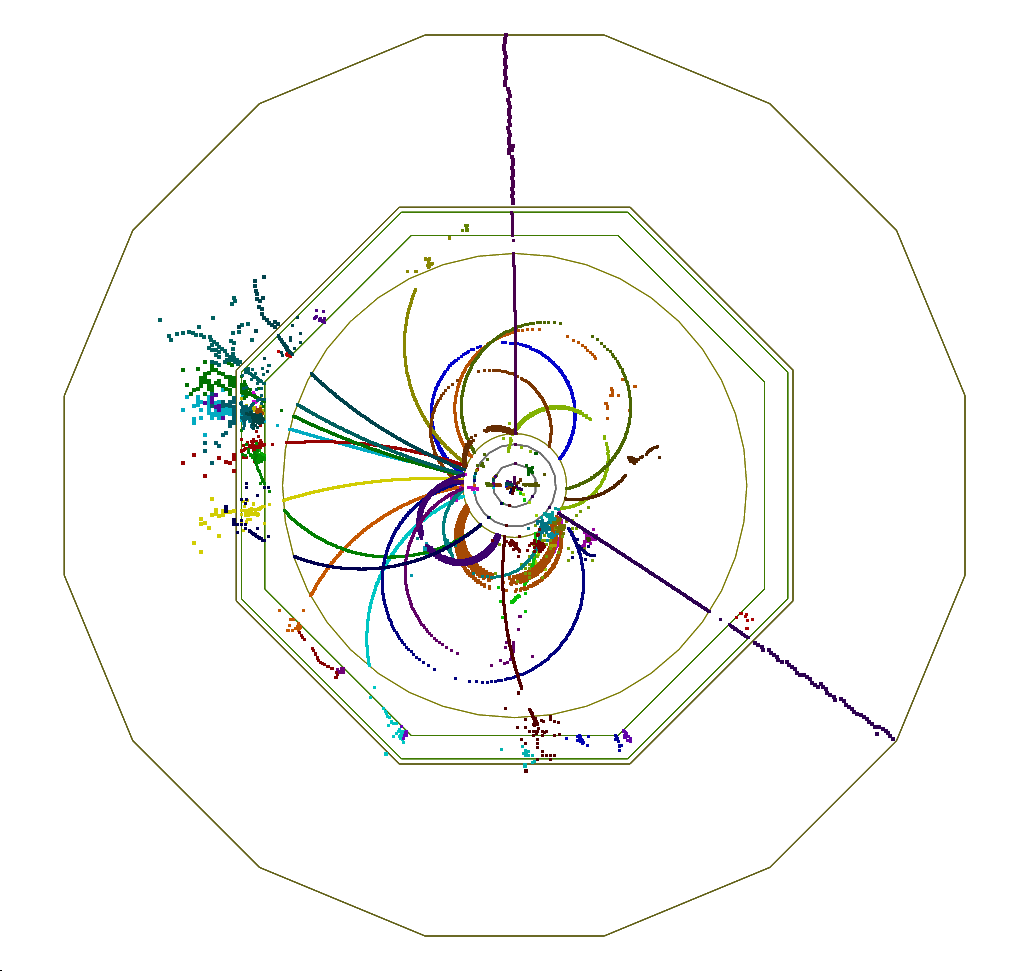
\includegraphics[height=0.65\textheight]{pr_frontview-70}};
          \node (img2) at (img1) {\only<2->{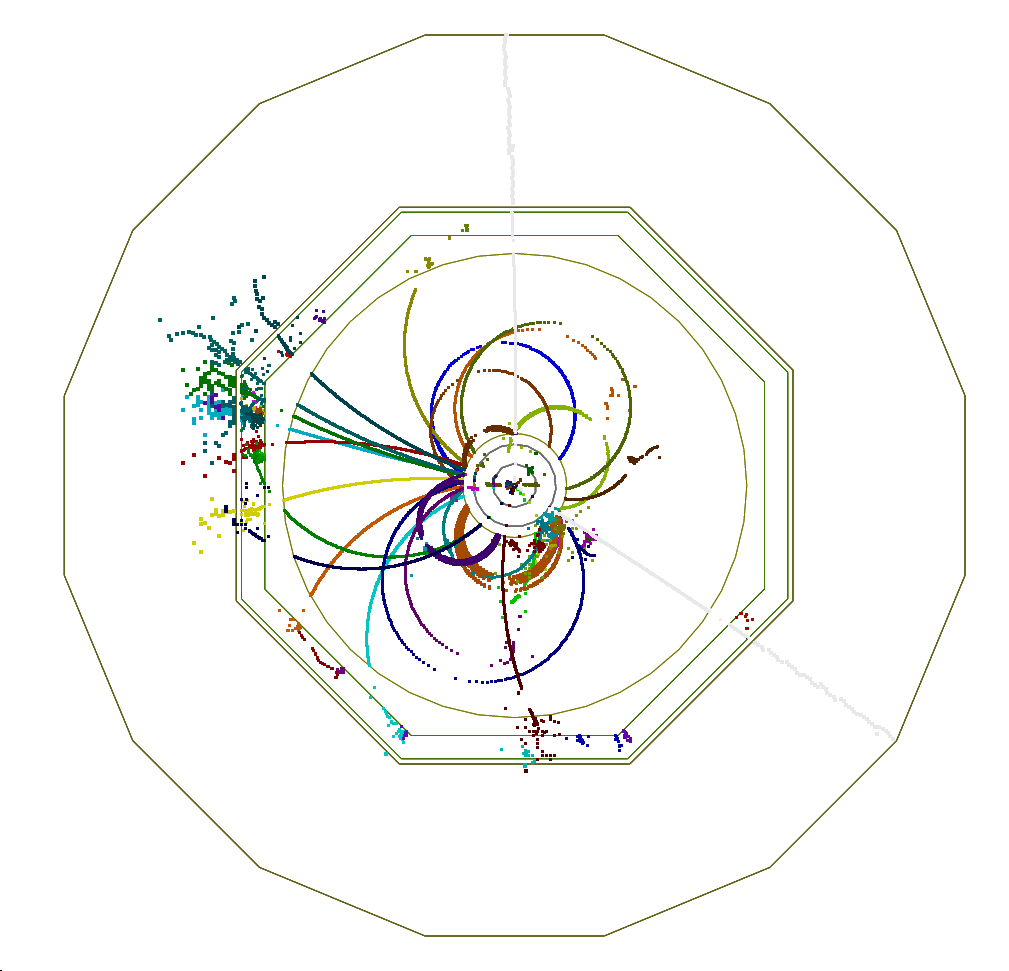
\includegraphics[height=0.65\textheight]{pr_frontview-70_noMu}}};
        \end{tikzpicture} &

        \begin{tikzpicture}
          \node (img1) {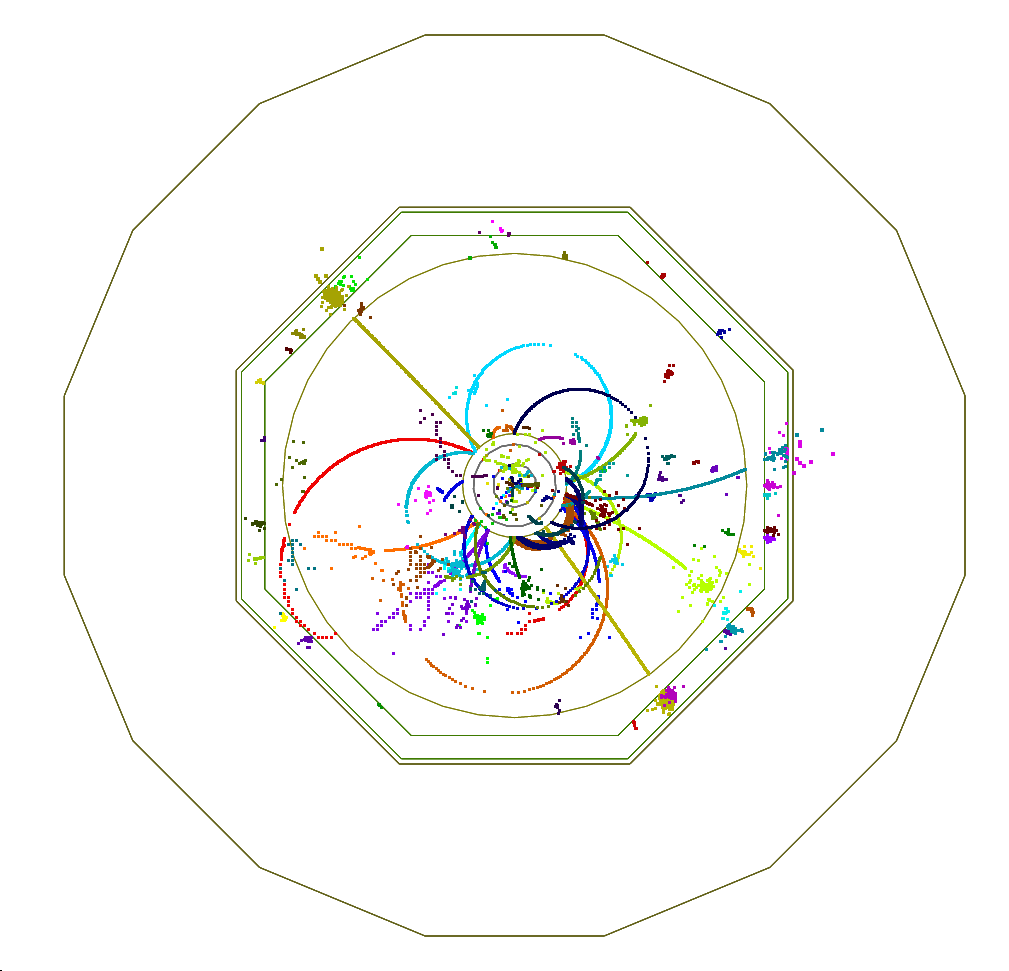
\includegraphics[height=0.65\textheight]{pr_frontview-91}};
          \node (img2) at (img1) {\only<3->{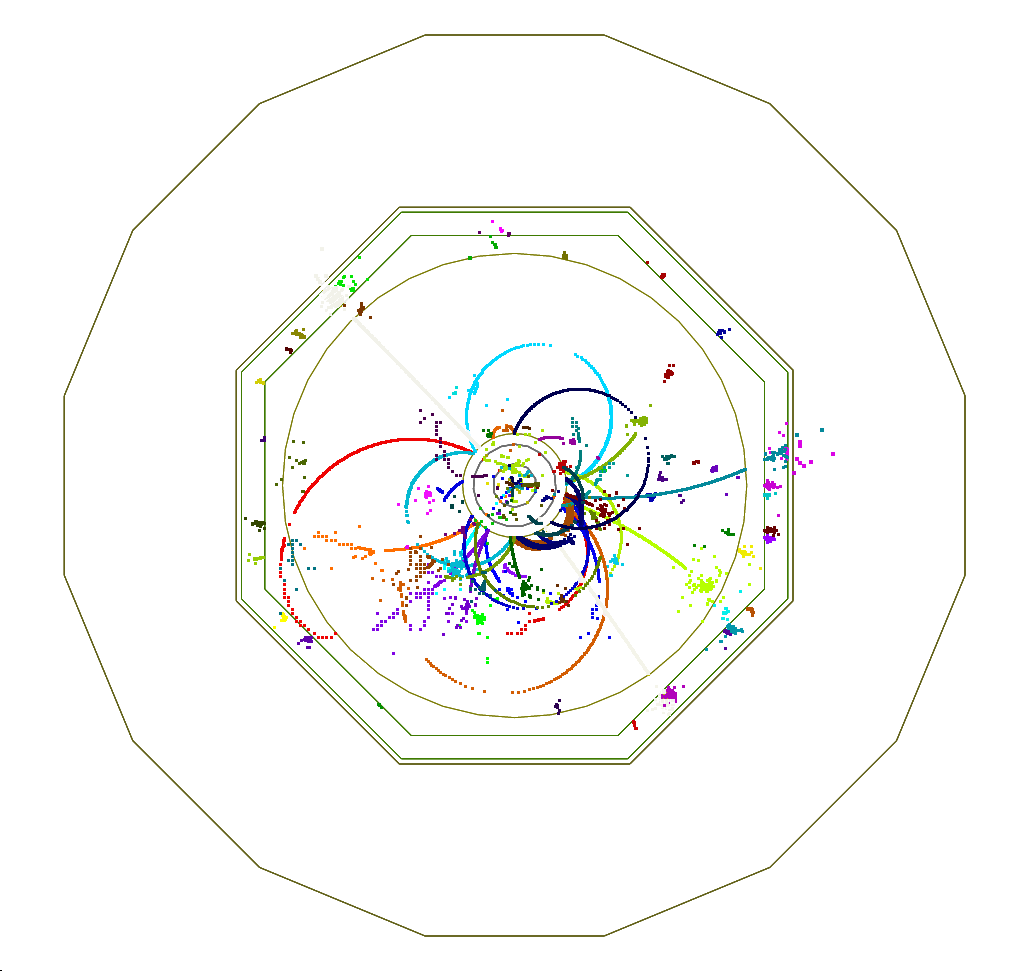
\includegraphics[height=0.65\textheight]{pr_frontview-91_noEl}}};
          \node (img2) at (img1) {\only<4->{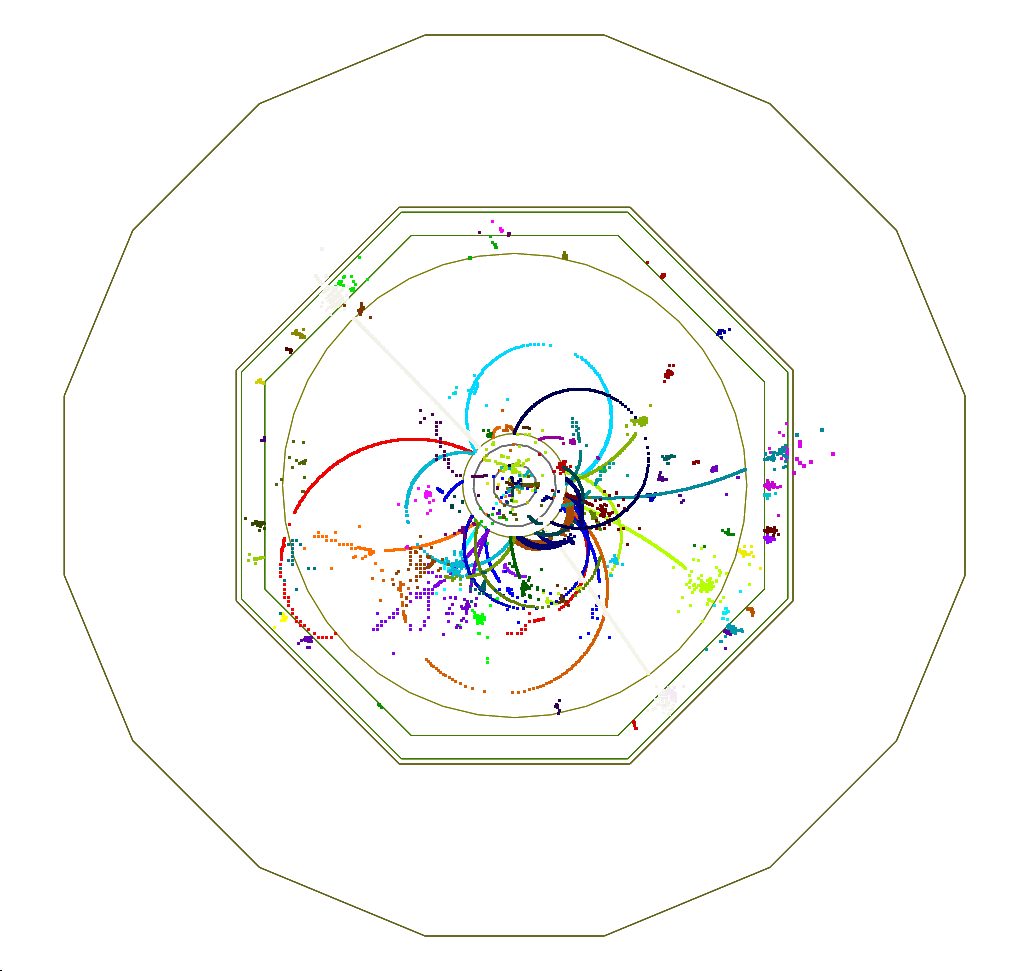
\includegraphics[height=0.65\textheight]{pr_frontview-91_noElGamma}}};
        \end{tikzpicture} \\
        \footnotesize{$e^+e^- \rightarrow H$
            \onslide<1>{$Z, \ Z \rightarrow \mu^+ \mu^-$}
        } &
        \footnotesize{$e^+e^- \rightarrow H$
            \onslide<-2>{$Z, \ Z \rightarrow e^+ e^-$}
        } \\
    \end{tabular}
    \end{frame}
